\documentclass[12pt,a4paper,openright,twoside]{book}
\usepackage[utf8]{inputenc}

\newcommand{\thesislang}{english}
\usepackage{thesis-style}

% version
\newcommand{\versionmajor}{0}
\newcommand{\versionminor}{1}
\newcommand{\versionpatch}{2}
\newcommand{\version}{\versionmajor.\versionminor.\versionpatch}

\begin{document}
	
\frontmatter

% ! TeX root = thesis-main.tex
\title{Title}
\author{Francesca Neri}
\date{\today}

\newgeometry{margin=0.8in}
\begin{titlepage}
	\begin{center}
		% \vspace*{0.2cm}
		
		\large
		\textbf{ALMA MATER STUDIORUM -- UNIVERSITÀ DI BOLOGNA \\ CESENA CAMPUS}
		\\
		\noindent\hrulefill
		\vspace{0.4cm}
		
		%\Large
		Department of Computer Science and Engineering - DISI \\
            \vspace{0.1cm}
        %\Large
		Second Cycle Degree in Digital Transformation Management \\
            \vspace{0.1cm}
            Class: LM-91
		
		\Large
		\vspace{4cm}
		\textbf{
			% The Role of Enterprise Performance Management \\ 
   %          in Modern Businesses: A Case Study of Oracle \\
   %          Cloud EPM Implementation
            Leveraging Oracle Cloud EPM Business Rules \\
            for Efficient Planning: Insights and \\
            Implementation Strategy
		}
		
		\large
		\vspace{2cm}
		Graduation thesis in \\
		\vspace{0.2cm}
		\textsc{BIG DATA AND CLOUD PLATFORMS}
		
		\vspace{5.5cm}
		\begin{minipage}[t]{0.64\textwidth}
			\begin{flushleft}
				Supervisor \\
				\vspace{0.2cm}
				\textbf{Prof. Matteo Francia}
			\end{flushleft}
		\end{minipage}
		\begin{minipage}[t]{0.34\textwidth}
			\begin{flushright}
				Candidate \\
				\vspace{0.2cm}
				\textbf{Francesca Neri}
			\end{flushright}
		\end{minipage}\\
		
		\vfill
		\noindent\hrulefill
		\vspace{0.3cm}
		\large
		
		I Graduation Session
		\\
		Academic Year: 2022-2023
	\end{center}
\end{titlepage}
\restoregeometry


\begin{acknowledgements}

This thesis is linked to my curricular internship for the final examination carried out at PricewaterhouseCoopers (PwC) from January to March 2023.
%
During the internship experience at PwC Italy, I worked in the advisory-transformation Line of Service, cooperating with the Enterprise Performance Management - Financial Service (EPM-FS) team.

The EPM-FS team works for the main players in the financial sector and deal with business transformation projects which are aimed at re-engineering and optimizing the company's internal processes.

Along the internship period, I worked directly with the EPM team in a project concerning the Oracle Cloud EPM platform.
%
This project is addressed to an Italian Corporate Group which has more than 7,000 points of sale around the world. 

Due to corporate policy, the name, data and information of the Corporate Group, to which the project is addressed, cannot be disclosed. 
%
It is important to note that respecting the privacy and confidentiality of companies' data is critical in maintaining their trust and credibility.
%
Therefore, throughout this thesis, I will be referring to the company only in general terms and avoiding the use of any identifying information or data.

I would like to express my gratitude to PwC Italy for this opportunity, to the entire EPM team for welcoming me and making me feel like a part of the team, and my supervisor for his guidance and support throughout the internship.

To be continued...

\end{acknowledgements}

\begin{abstract}	

This thesis explores the role of Enterprise Performance Management (EPM) solutions in modern businesses, ranging from planning, reporting and forecasting purposes. 
%
The project was carried out using Oracle Cloud EPM, a cloud-based platform developed by Oracle Corporation, that offers an integrated suite of financial and operational planning and analysis tools.

The thesis starts by providing an overview of Enterprise Performance Management and its importance in modern businesses. 
%
It then delves into the benefits of using a cloud platform for EPM, including lower costs, increased flexibility, and easier scalability.

The main focus of the thesis regards the exploration of how financial and operational processes are integrated in a single EPM solution, whilst using data coming from different sources. 
%
The project involved working with a real-world client to identify the company planning needs and
then manipulating dimensions, elements, and hierarchies to meet those needs.
%
The techniques used to create customized planning models for the client will be analyzed, including the use of pre-built templates and the creation of custom calculations and formulas.

In addition to the technical aspects of the project, this thesis also explores the business benefits of using an integrated EPM solution, including better decision-making, improved financial performance, and increased visibility into operational processes.

Overall, the goal of this project is to provide a detailed exploration of the role of EPM solutions in modern businesses, with a focus on the importance of using a cloud platform and integrating financial and operational processes in a single solution. 
%
The project, carried out using Oracle Cloud EPM, provides a practical example of how businesses can leverage EPM solutions to improve their financial and operational planning and analysis capabilities.

\end{abstract}

\begin{dedication}
Optional. Max a few lines.
\end{dedication}

% \begin{acknowledgements}
% Optional. Max 1 page.
% \end{acknowledgements}

%----------------------------------------------------------------------------------------
\tableofcontents   
%\listoffigures     % (optional) comment if empty
%\lstlistoflistings % (optional) comment if empty
%----------------------------------------------------------------------------------------

\mainmatter

%----------------------------------------------------------------------------------------
\chapter{\introductionname}
\label{chap:introduction}
%----------------------------------------------------------------------------------------

In today's highly competitive business environment, effective performance management is essential for organizations to achieve their strategic goals and stay ahead of the competition.
%
With the advent of digital transformation, companies are now offered with huge opportunities from which they can benefit.
%
It is an inevitable change that organization must embrace to stay competitive and meet customer demands in the digital era.

One of the way to go in order to thrive among rivals in turbulent markets is to excel at various performance dimensions. 
%
One of the prerequisites for this is to be able to effectively manage and measure corporate performance using various performance management and measurement systems. 
%
These systems help companies to continuously react and adapt to external changes.

Enterprise and corporate performance and management methods can be viewed as the seamless integration of managerial systems. 
%
Each method should be embedded with business analytic operations like correlation, segmentation, regression and predictive analysis.
%
Performance management provides valuable data and insights that can help businesses make informed decisions by identifying trends, anticipating issues, and making adjustments to their strategy as needed.

Enterprise Performance Management (EPM) is an integral part of the success of modern enterprises as it helps organizations to gain visibility into their performance and to identify areas of improvement.
%
It is a management approach that integrates multiple business processes and systems to enable organizations to plan, measure, analyze, and optimize their performance.

 Enterprise Performance Management enables businesses to improve strategic decision-making, maximize their productivity and achieve the desired business results while ensuring that expenses are minimized and that the best use of resources is made.
 %
 It assists businesses to effectively forecast and plan for their future financial performance, helping them to ensure compliance and reduce risk. 
 
 The advantages of EPM are numerous and make it a valuable tool for organizations of all sizes.

 The aim of this thesis is to investigate the role of EPM in modern businesses and the benefits and challenges of implementing EPM solutions. 
 %
 Specifically, this thesis will focus on a case study of Oracle Cloud implementation in a business to illustrate how EPM solutions can improve organizational performance. 
 
 Oracle Cloud is a leading cloud-based EPM solution that provides organizations with a comprehensive suite of financial and operational performance management applications.
 %
Oracle Cloud EPM provides a flexible and scalable solution that can meet the needs of organizations of all sizes.
%
It offers various tools and solutions that allow companies to plan, budget, forecast, and report on their financial and operational performance.
%
The implementation of an Oracle Cloud EPM solution involves a series of steps throughout which organizations must work closely with their implementation partner to ensure that the solution is tailored to their specific needs and requirements.

Using a cloud platform to implement an EPM solution can provide numerous benefits for the organization. 
%
One of the primary advantages regards the ability to access critical data and applications from anywhere and at anytime.
%
Additionally, cloud platforms can help reduce costs associated with maintaining on-premises infrastructure and provide scalability and flexibility to meet changing business needs. 
%
Cloud-based EPM solutions also enable organizations to leverage the latest technologies and innovations without having to worry about managing and upgrading hardware and software. 
%
Cloud providers typically offer high levels of security and compliance, which can help organizations protect sensitive data and maintain regulatory compliance. 

%
\paragraph{Thesis Structure.}
%

Accordingly, the reminder of this thesis is structures as follows:
%
\Cref{chap:introduction} will provide an overview of the background and significance of the topic, scope and limitations of the study, and an overview of the methodology.
%
\Cref{chap:background} will review the literature on Enterprise Performance Management, including the definition and concepts of EPM and its evolution in modern businesses. 
%
It also provides an overview on Oracle Cloud and its EPM solutions, together with the benefits and challenges of implementing EPM in businesses. 
%
\Cref{chap:design} will describe the approach and methodology used for the implementation of and EPM solution to a company.
%
\Cref{chap:implementation} will present the case study of Oracle Cloud implementation in a business, including the company background and context, EPM solution selection and implementation process, key features and functionalities of the implemented EPM solution, impact of the EPM solution on the company's performance, and the best practices for EPM implementation. 
%
Finally, \Cref{chap:conclusions} concludes the thesis summarizing the main concepts ans discussing the implication for theory and practice.

\section{Background and significance of the study}

Enterprise Performance Management is a management approach that involves using data and analytics to monitor, measure, and improve an organization's performance. 
%
It integrates various management processes, including financial planning, budgeting, forecasting, risk management, and performance measurement, to help organizations align their goals with their strategies and improve their overall performance.
%
To access and analyze data more quickly and accurately, organizations typically use software applications that automate and streamline this process.

These application often include dashboards, pre-built report templates and other tools that provide real-time insights into organizational performance.

The ultimate goal of EPM is to help organizations to achieve their strategic objectives and optimize their performance, whether that be in terms of financial performance, customer satisfaction, operational efficiency, or other key performance indicators. 
%
By using data-driven insights and decision-making, EPM enables organizations to more effectively manage risks, allocate resources, and make strategic decisions that improve their overall performance and competitiveness in the marketplace.

Enterprise Performance Management operates within a complex and dynamic business environment, characterized by a number of key trends and challenges. 
%
One of the most significant trends in recent years has been the growing adoption of cloud technology for enterprise applications, including EPM. 

Cloud-based EPM solutions offer many advantages over traditional on-premises systems, including greater scalability, flexibility, and accessibility, as well as lower costs and reduced IT complexity. 
%
As a result, more and more organizations are turning to cloud-based EPM solutions to improve their performance management processes.

Another key trend in modern business is the growing importance of data-driven decision making. 
%
With the increasing availability of data and advanced analytical tools, organizations are able to gain deeper insights into their operations and performance, and make more informed decisions. 
%
EPM plays a critical role in this trend by providing real-time insights into organizational performance and enabling managers to make data-driven decisions that align with their strategic goals. 
%
This helps organizations to be more proactive in identifying and responding to performance issues, and to optimize their operations and resources to achieve their desired outcomes.

In addition to these trends, EPM also operates within a business environment that is constantly evolving and adapting to changing market conditions. 
%
The need for businesses to be agile and responsive to these changes is an ongoing challenge, and EPM can help address this by providing a flexible and adaptable framework for performance management. 
%
By monitoring key performance indicators and providing real-time insights into performance, EPM enables businesses to quickly identify and respond to changes in market conditions, and to make strategic decisions that keep them ahead of the competition.

Overall, the context in which EPM operates is characterized by a rapidly evolving business environment, where technology, data, and agility are critical to success. 
%
Enterprise Performance Management plays a critical role in helping organizations to adapt to these trends and challenges, by providing a data-driven and agile approach to performance management that enables them to optimize their operations, resources, and strategic decision making.

\section{Scope and limitations of the study}

The scope of the project includes different areas of focus that range from the definition of Enterprise Performance Management, its benefits, its implementation in companies and the future trends.
%
The thesis starts by defining what Enterprise Performance Management is and how it differs from the other management approaches in place.

Then, the project investigates the potential benefits that EPM can bring to modern businesses including enhanced decision-making, better alignment of business objectives with strategies, increased efficiency and improved performance.
%
It then explores the challenges associated with implementing EPM solutions in businesses which, for example, include issues related to data collection and analysis, performance measurement, reporting and the use of technologies and specific software.
%
Data is the core element of a performance management system; in order to have accurate reports and effective forecasts, it is important to have large quantities of data which which the EPM system is populated. 

The project aims at analyzing a case study regarding the implementation of an EPM solution in a company.
%
Then, it explores the future trends and challenges that are likely to impact the role of Enterprise Performance Management in relation with emerging technologies, changing business models, and evolving business needs and expectations.

There are some limitations related to the study that should be taken into account.
%
Such limitations include both extrinsic and intrinsic elements of the project, ranging from the access to large amounts of data, the complexity of the topic investigated and the diversity of applications involved.

More in details, in order to explore the impact of Enterprise Performance Management on businesses, it may be necessary to have access to data related to business performance belonging to different organizations.
%
However, in this thesis we will analyze a case of implementation carried out for a specific company which operates in a specific industry sector. 
%
Of course, each company has its own characteristics in terms of operations and business management, which impact the implementation of the solution and its overall effectiveness.
%
Also, modern businesses vary widely in terms of size, sector, business model and many other factors.
%
In particular, the activities of management and performance control carried out by the company have a significant impact on how the EPM solution will be implemented and maintained.
%
Of course, there is no single solution that can be applied to any business but they vary according to the needs of the company.
%
As a result, it can be difficult to generalize findings in one type of business to other types of businesses.

\section{Overview of the methodology}

The methodology applied to the implementation of an Enterprise Project Management solution follows some key steps and best practices that depend on the specific requirements of the client company, the size and complexity of the project and the available resources.
%
The entire implementation process is built together with the client company which is responsible for assessing the quality of each step and ensuring the compliance with the requested features of the system.

The project begins with a planning phase, during which the company's business needs and goals are identified and the scope of the project is defined.
%
This involves identifying the objectives and key deliverables of the project, as well as any constraints or assumptions that will impact the implementation.
%
During this phases, it is important to identify the stakeholders by determining who will be impacted by the implementation and what their needs and requirements are.
%
Another key element in the planning phase is the definition of success criteria in order to measure the outcome by using performance indicators.
%
Finally, a clear and detailed project plan is developed, outlining the timeline, the budget, and resources required to complete the implementation.

Then, during the solution design phase, the EPM solution is designed based on the identified business requirements and goals, including the configuration of the environment, customizing features and workflows, and integrating with other systems.

The development and testing phase is the core part of the project.
%
In this phase the EPM solution is built and configured, relying on a process of continuous feedback from the customer.
%
Both individual components and the solution as a whole are tested to ensure that they meet the business requirements and goals.

After that, the client company's personnel which will use the system is trained through training sessions, user manuals, and other resources to help users understand the system and use it effectively.

Finally, the solution is deployed to the client's company environment.
%
If applicable, the data of the old system will be migrated into the new one, which will be integrating with additional existing systems.
%
After the EPM solution is deployed, configured and permissions are set, ongoing support and maintenance are provided to ensure the system runs smoothly and meets the company's needs.
%
This involves providing technical support, troubleshooting issues, and applying updates to keep up with the software advancements.

%----------------------------------------------------------------------------------------
\chapter{Literature Review}
\label{chap:background}
%----------------------------------------------------------------------------------------

Write background here.

This section is likely to contain a lot of citations.

\section{Definition and concepts of Enterprise Performance Management}

\section{The evolution of EPM in modern businesses}

\section{Oracle Cloud and its EPM solutions}

\section{Benefits and challenges of implementing EPM in businesses}

%----------------------------------------------------------------------------------------
\chapter{Methodology}
\label{chap:design}
%----------------------------------------------------------------------------------------

% \begin{figure}
% 	\centering
% 	\includegraphics[width=0.5\linewidth]
% 	\caption{A class diagram created with PlantUML}
% 	\label{fig:classes}
% \end{figure}

The successful implementation of an enterprise performance management (EPM) system can have a significant impact on the performance and competitiveness of modern businesses. 
%
However, the implementation of such a system requires careful planning, preparation, and execution to ensure success. 

In the case of Oracle Cloud EPM, a comprehensive methodology is needed to guide the implementation process from planning and scoping to go-live and ongoing support.

In this section, we will examine the methodology used in the implementation of a Oracle Cloud EPM solution for a company.
%
We will discuss the key steps involved in the implementation process, including planning and scoping, system design and configuration, data integration and migration, testing and validation, training and change management, and go-live and ongoing support. 

We will also explore specific approaches, methodologies, and tools used in each phase of the project, and discuss the challenges and lessons learned throughout the implementation. 
%
By examining the methodology used in this project, we can gain insights into best practices for Oracle Cloud EPM implementation and its unique features and tools.

\section{Scope and objectives of the project}

This project is addressed to an Italian Corporate Group which has more than 7,000 points of sale around the world. 
%
An Enterprise Performance Management implementation project involves the deployment of a software solution that will enable the company to effectively manage its financial data, analyze it, and make informed business decisions.

The goal of the project is to implement a planning environment in Oracle Cloud EPM in which the data belonging to the different brands of the group are all integrated in a single view.

In particular, the planning environment is used an maintained by the client's management control department so, along the implementation process, we interacted directly with the people working in that area.

The Corporate Group was born in 2018 and is the result of the aggregation of different companies which belong to the same industry sector.
%
The entities which compose the Group have a different story, a different culture, different business models and, as a consequence, different Group Control Models.

Since its creation, the new Group has planned several initiatives to facilitate the integration between the different realities.
%
The lack of organizational structure due to the different Group Control Models was considered as a key issue in sustaining the new planning and reporting needs of the Group.
%
To solve this issue, the Group started an activity of  homogenization of Enterprise Performance Management model of the entities, by:

\begin{enumerate}
    \item Defining a consolidated financial reporting:
    \item Defining a performance reporting system based on KPI’s;
    \item Defining a treasury reporting and rolling cash flow forecast process;
\end{enumerate}

The objective of the client company is that of gaining visibility and control over the Group performance with an homogeneous and consolidated reporting activity.
%
They plan to achieve a deep visibility on the companies performances, in order to extract insights and KPIs from entities independently.

At the same time, the companies which are part of the group necessitate a clear consolidation process and homogeneous reporting.
%
For them, it is important to achieve high reliability on data and reporting, thus enhancing data quality, as well as enlarging the Enterprise Performance Management model at entity level to extract analytics locally.

The project implementation goes around two main macro-areas which are: financial and management reporting and performance analysis.
%
Financial reporting and analysis are mandatory for businesses and are mainly used for external purposes.
%
Financial reports include:

\begin{enumerate}
    \item Profit and Loss Statement;
    \item Income Statement;
    \item Balance Sheet;
    \item Accounts Payable;
    \item Accounts Receivable;
    \item Statement of Cash Flows;
\end{enumerate}

These reports are important for stakeholders like banks, investors and regulators, to ensure that the company is following accounting standards correctly.
%
Financial reporting reflects the financial position of a business at the time of reporting, however, they cannot be used to predict future performance or provide insights.

Management reporting is optional and is for internal business purposes. 
%
Management reports aim to dive deeper into the company financials and provide insights that enable more informed business decisions. 
%
These reports include:

\begin{enumerate}
    \item Profit and loss by category (team, job, department);
    \item Inventory reports;
    \item Sales reports;
    \item Utilisation reports;
\end{enumerate}

Management reporting focuses on individual areas of the business, allowing companies to identify areas that are strong and any area of potential improvement. 
%
For example, they might want to see how well the sales department is performing one month before making the decision to expand. Management reporting for performance management enables leaders to rely on their numbers.

Performance analysis, on the other hand, is the process of evaluating the performance of a business, product, service, or process against established benchmarks and objectives. 
%
It involves collecting and analyzing data to identify patterns, trends, and opportunities for improvement.

Performance analysis is particularly important for businesses because it helps them to identify areas of strength and weakness, improve efficiency and productivity, reduce costs and waste, increase revenue and profitability, enhance customer satisfaction and stay competitive in the market.
%
Financial reports can be used to assess different areas of a business and provide valuable insights into its performance.

Then, in terms of people and organization, the goal of the project is to define the financial organization process at Holding level in order to manage all processes in line with the Group Control Model.
%
Processes are defined at the Group level, based on their best practices, while the financial organization process is reviewed at entity level with different prioritization, in order to align the needs of the Group Control Model.

\section{Project plan and needs assessment}

A project plan is a comprehensive document that outlines the key objectives, milestones, tasks, timelines, and resources required for the successful completion of a project. 
%
It is an essential tool for project management, as it provides a road-map for project execution and allows for effective tracking and monitoring of progress.

Project plans help to define the scope and objectives of the project, identify the specific tasks and activities required to achieve the project objectives and determine the timelines and milestones for each task and activity.

At an operational level, designing a precise project plan allow for the effective allocation of the necessary resources, such as budget, personnel, and equipment, to complete the project.
%
At the same time, it ensure effective communication and collaboration between team members while facilitating the tracking and monitoring of progress towards project goals.
%
You can go back to them and check what you said you were going to do and how, comparing it to what you are actually doing. This gives a good reality check and enables to change course if needed, bringing the project back on track. \\

The needs assessment is a systematic process for determining and addressing needs and requirements to fill the gap between the current conditions and the desired conditions.
%
This process should be undertaken before the project work begins, therefore, it belongs to the initiation phase.

The goal of this initial phase is to assess the current financial reporting and analysis process used by the company to identify pain points, inefficiencies and areas of improvement.
%
The key steps carried out during the process, include:

\begin{enumerate}
    \item Requirements: Understanding everything that is involved with the project, ensuring that the project’s context and objectives are clear. By understanding the specifics, it is easier to identify the needs associated with the project, as well as explaining individual milestones and deliverables to the people involved to provide a broader context.
    \item Resources: Match the existing, available resources to what is needed to perform the project. 
    \item Gaps: Once the resources have been identified, we can truly address the ones that are not already fulfilled. This way, we will make sure to uncover and address any gaps, which can vary from a particular skill set to the software needed to execute a task. 
    \item Create a plan to fill the gaps: Once all the gaps have been successfully identified, we can use this information and address these issues by designing a plan of action. 
\end{enumerate}

Overall, the needs assessment phase is critical in ensuring that a project is aligned with the needs of its intended beneficiaries, and that it is designed to meet their needs and address the specific problem or opportunity effectively.
%
Before starting an EPM implementation project, it is important for a company to conduct a thorough need assessment to ensure that the project aligns with its objectives and addresses its most pressing needs.

\section{Project requirements}

For a Holding Group whose goal is to design and maintain a comprehensive and integrated planning solutions to monitor the performance of all the brand that are part of the Group, we can identify several key requirements to be considered in order to ensure a successful implementation:

First of all, the EPM system should allow for centralized data management, ensuring that data can be collected, consolidated, and analyzed across all brands.
%
It is of key importance to define some common standards that need to be followed by the brands in order to integrate data smoothly.
%
More in details, to obtain an integrated view on the brands' performance, entities should adopt technologies that bring data together from across the business ecosystem to create a single, accurate and transparent record of the truth.

Such solution is known as Master Data Management and is the core process used to manage, centralize, organize, categorize, localize, synchronize and enrich master data according to the business rules of the controlling Group.
%
The efficient management of master data in a central repository allows for a single authoritative view of information and eliminates costly inefficiencies caused by data silos.
%
It supports business initiatives and objectives through identification, linking and syndication of information and content across products, customers, stores/locations, employees, suppliers, digital assets and more.

Then, the EPM system should provide flexible and customizable reporting capabilities that can be tailored to the needs of each brand.
%
At the same time, the system should be easy to use for employees across all brands, with an intuitive interface that requires minimal training.

Moreover, it should be able to integrate seamlessly with existing systems used by the holding group and its brands, such as ERP (Enterprise Resource Planning) and CRM (Customer Relationship Management) software.
%
By all means, the system should be scalable to accommodate future growth and expansion of the holding group and its brands.

\begin{figure}[ht]
	\centering
	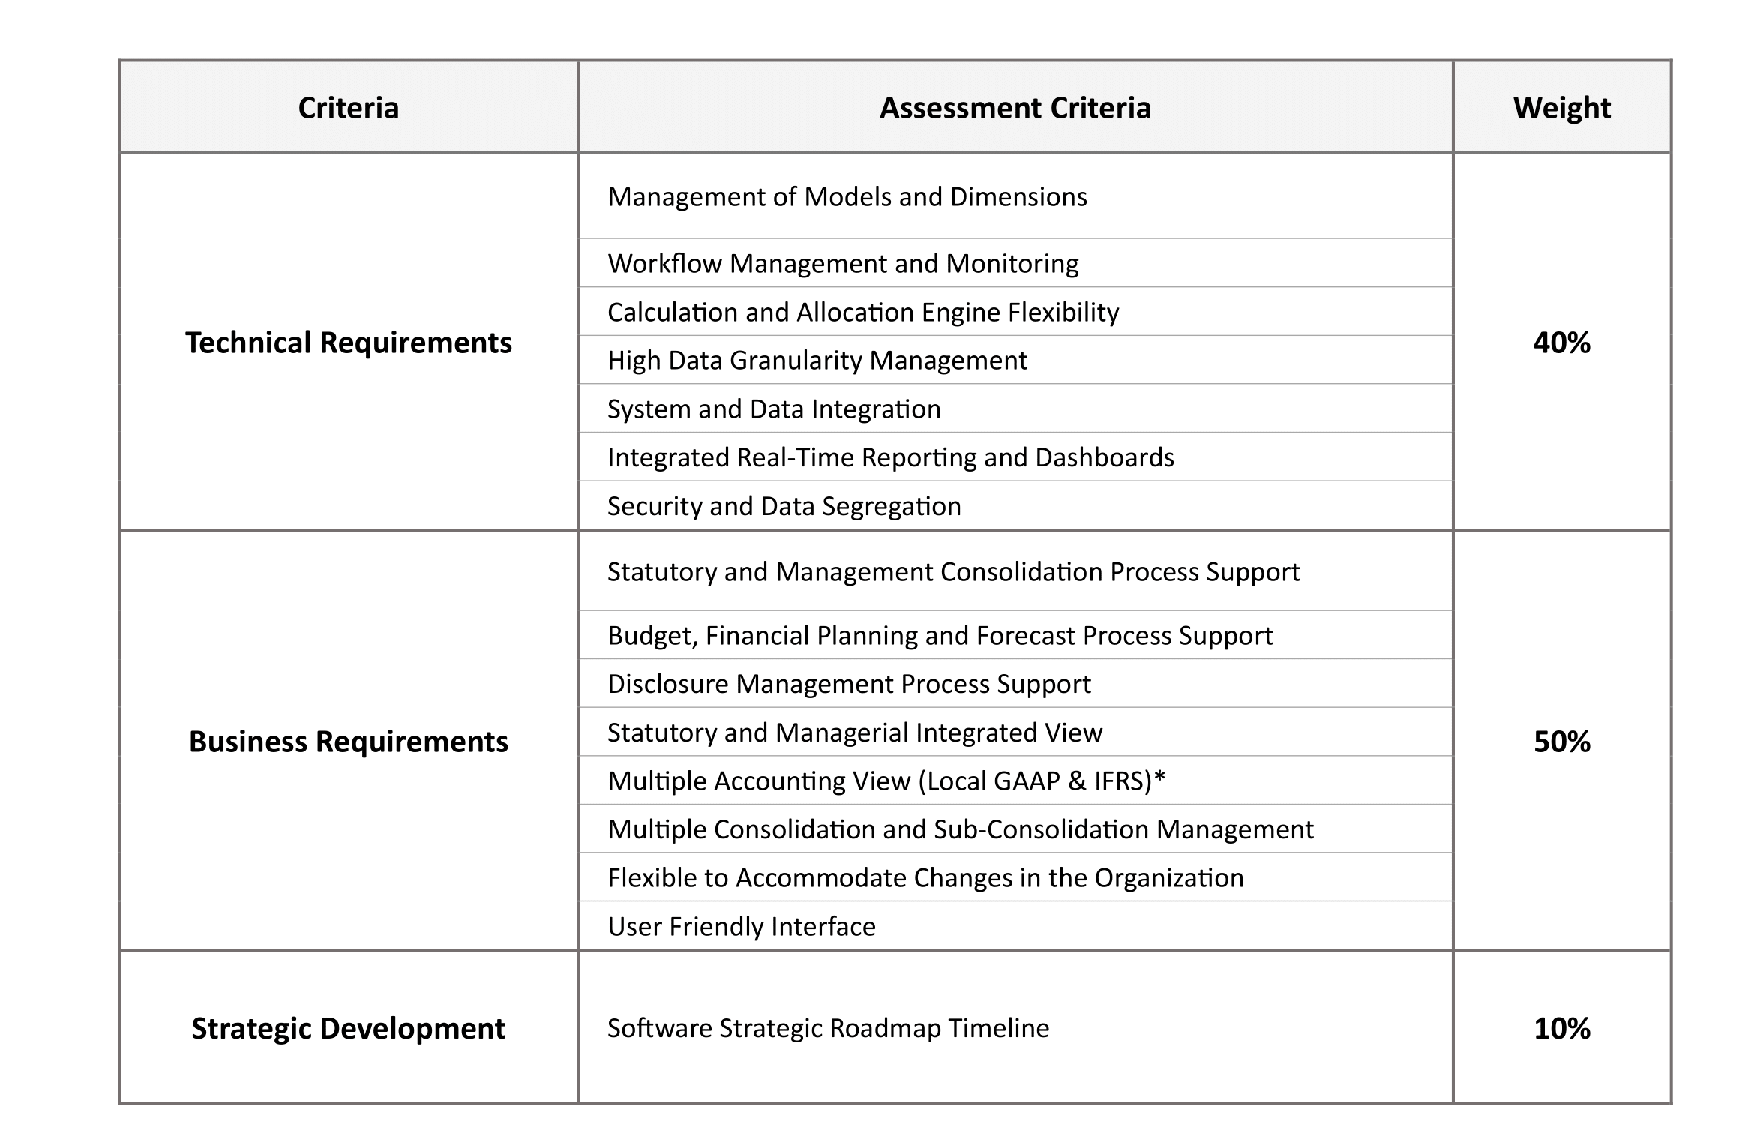
\includegraphics[width=\linewidth]{figures/requirements.pdf}
	\caption{Technical, Business and Strategic Requirements}
	\label{fig:requirements}
\end{figure}

Figure \ref{fig:requirements} lists all the technical, business and strategic requirements that should be considered when choosing the right tools and technologies for the implementation of the EPM solution.
%
It is important to identify and prioritize both business requirements and technical requirements when planning an EPM implementation project, in order to build an effective and maintainable solution.

Technical requirements cover the specific features and capabilities that the system must have in order to ensure that the EPM system is effective, reliable, and able to meet the unique needs of the Group and its entities.
%
More in details, the use of technologies that allow for integrated modeling that is easy-to-maintain and with no limitations of dimensions is of key importance for this project.

For example, a Holding Group which owns different brands and entities across the globe may need to frequently update the \textit{Product} or \textit{Geography} dimension every time they add a new product or sell to a new country.
%
At the same time, users need to have a clear and structured workflow of activities that supports them in the use of the EPM system, while the Control Group should be able to track and monitor the progress of single activities carried out by the entities.

Then, in terms of calculation and allocation flexibility, we refer to the possibility to perform custom calculations and extend predefined rules (like consolidation and currency translation), in order to meet the specific needs and requirements of each entity.
%
The system should also be able to manage data of different granularity as the level of detail and precision in data structures depends on the activity to perform.
%
The EPM platform needs to manage high-volume data and possibly interface with big data systems.

Naturally, system and data integration must be available.
%
In particular, the system should have an integrated solution for ETL (Extract, Transform and Load) activities, completed with advanced mapping features to accommodate multi-source and multi-ERP loading.

Reporting and dashboarding can be setup ``live'' for all data available in the interconnected solution
applications to enable the group to make informed decisions based on its financial data.

Finally, the EPM system should have robust security features to protect sensitive financial data, while allowing the Control Group to manage granular securities at the micro-detail of data to handle the read and write permissions of the different entities.

Business requirements, on the other hand, regard the specific goals, needs, and expectations of the stakeholders and users of a system. 
%
In our context of EPM implementation project for a Holding Group, business requirements are set to reach key business goals, like streamlining financial reporting, improving decision-making based on financial data, increasing efficiency and accuracy in budgeting and forecasting, and providing a centralized system for financial management across all entities. 

One of the key priorities for a Holding Group is to have a clear statutory and consolidation process with the possibility to adopt multiple consolidation methods, including full consolidation, proportionate consolidation, and equity consolidation.
%
Consolidation accounting is the process of combining the financial results of several subsidiary companies into the combined financial results of the parent company as though they were a single firm.

The system should have predefined modules to address different planning standard processes and an open ``free from'' planning mode to create personalized planning environments. 
%
At the same time, it should include embedded predictive planning, risk based planning and strategic  long-term modeling feature.

Public companies must prepare disclosure reports for internal and external stakeholders to shine a light on the company's performance and operating activities.
%
Disclosure reports contain information about a company's business activities, financial condition, management compensation, operating performance and future direction. 
%
It is therefore essential for the EPM system to provide disclosure management functionalities to help the Group to fulfill the disclosure requirements of regulators like the Security and Exchange Commission or the European Central Bank.

The system should provide  a unified environment able to guarantee the consistency and coherence of data generated at each level of the statutory, management and disclosure reporting.
%
In this regard, users should be able to compare multiple accounting views depending on the country of interest (GAAP for United States and IFRS world-wide).

Finally, the EPM system should be flexible enough to adapt to changing business needs and requirements, allowing for an easy-to-use, adjustable interface that every user can use to create different versions of reports, depending on the current need.

Making architecture changes or modifying operations takes a clear plan of where the organization is, where it wants to go, and how to get there. 
%
A strategic road-map lays out the direction of IT efforts that span across an organization in a simple way to align teams and key stakeholders.
%
The implementation of the EPM solution should be in line with the company's strategic road-map, both in terms of deliverables and process schedule and timing.

%----------------------------------------------------------------------------------------
\chapter{Case Study: Oracle Cloud Implementation}
\label{chap:implementation}
%----------------------------------------------------------------------------------------

\section{Company background and context}

%Add technical requirements from DH slides

\section{EPM solution selection and implementation process}

\section{Key features and functionalities of the implemented EPM solution}

\section{Impact of the EPM solution on the company's performance}

\section{Best practices for EPM implementation}

%----------------------------------------------------------------------------------------
\chapter{\conclusionsname}
\label{chap:conclusions}
%----------------------------------------------------------------------------------------

\section{Summary of the project}

\section{Discussion and concluding thoughts}


%----------------------------------------------------------------------------------------
% BIBLIOGRAPHY
%----------------------------------------------------------------------------------------

\nocite{*} % uncomment this to show all the reference in the .bib file
\bibliographystyle{plain}
\bibliography{bibliography}


\end{document}